\begin{problem}{/images/problems/pic.jpg}{Long Loop}What is the output of the following code?

\begin{center}
	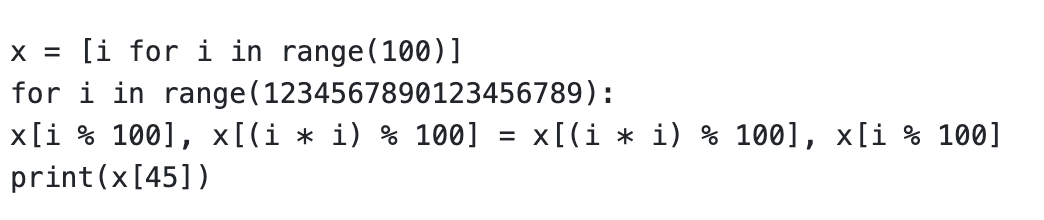
\includegraphics[width=9cm]{/images/problems/22_code.png}
\end{center}

Link to the problem on Twitter:  \url{https://twitter.com/Riazi_Cafe/status/1688797212602667008}\end{problem}
\begin{solution}
The answer to the problem is equal to 65.\\[0.2cm]

The first observation is that only numbers that end with digit 5 will be moved to positions that end with digit 5. Therefore, it suffices to only consider 10 numbers $5, 15, \ldots, 95$ in the sequence.
During the first 100 operations of the for loop, the position of these numbers changes as follows:

$$5 \rightarrow 15 \rightarrow 35 \rightarrow 45 \rightarrow 55 \rightarrow 65 \rightarrow 75 \rightarrow 85 \rightarrow 95 \rightarrow 25 \rightarrow 5.$$

Since the length of this cycle is 10, we return to the initial state by repeating these changes 10 times. In other words, after 1000 operations of the for loop, the positions of these numbers return to the initial state. Therefore, it is sufficient to solve the problem for the case where the size of the for loop is equal to 789, in which case the answer to the problem is equal to 65.



\end{solution}
